\documentclass[12pt]{article}
\usepackage{amsmath}
\usepackage{amssymb}
\usepackage{geometry}
\usepackage{enumerate}
\usepackage{natbib}
\usepackage{float}%稳定图片位置
\usepackage{graphicx}%画图
\usepackage[english]{babel}
\usepackage{a4wide}
\usepackage{indentfirst}%缩进
\usepackage{enumerate}%加序号
\usepackage{multirow}%合并行
\title{\large UM-SJTU JOINT INSTITUTE\\PHYSICS LABORATORY\\(VP141)\\\ \\\ \\\ \\\ \\\ \\\ \\\ \\\ \\\ \\\ \\\
LABORATORY REPORT\\\ \\\ EXERCISE 2\\\  Measurement of the Fluid Viscosity \\\ \\\ \\\ \\\ \\\ }
\author{Name: Pan Chongdan\\ID: 516370910121\\Group: 16}
\date{Date: \today}

\begin{document}
\maketitle
\newpage
\section{Introduction and Theoretical Background}
\subsection{Objectives}
In this exercise I'll get familiar with the constant-torque method for measuring the fluid viscosity, which is one of the most important properties of fluids, determining the fluid's flow. Student will learn Stokes' method, which is a common and simple method for characterizing transparent and translucent fluids with high viscosity.
\subsection{Basic Concepts of Fluid's Viscosity}
The viscosity of a fluid is a measure of its resistance to gradual deformation by shear stress or tensile stress. For liquids, it corresponds to the informal concept of "thickness"; for example, honey has a much higher viscosity than water.
\par Viscosity is a property of the fluid which opposes the relative motion between the two surfaces of the fluid in a fluid that are moving at different velocities. When the fluid is forced through a tube, the particles which compose the fluid generally move more quickly near the tube's axis and more slowly near its walls; therefore some stress (such as a pressure difference between the two ends of the tube) is needed to overcome the friction between particle layers to keep the fluid moving. For a given velocity pattern, the stress required is proportional to the fluid's viscosity.
\par Fluid's viscosity only determined by its type and temperature.
\section{Measurement of Fluid's Viscosity}
Motion of an object in a fluid is hindered by a drag force acting in the direction opposite to the direction of motion,for example, opposite to the object's velocity. The magnitude of the drag force is related to the shape and speed of the object as well as to the internal friction in the fluid. This internal friction can be quantified by a number known as the viscosity coefficient $\eta$
\par For a spherical object with radius $R$ moving at speed $v$ in an infinite  volume 
of a liquid, the magnitude of the drag force is usually modeled as linear in the speed
\begin{equation}
F_1=6\pi{\eta}vR
\end{equation}
When a spherical object falls vertically downwards in a fluid, it is being acted upon by the following three forces: The viscous force \textbf{$F_1$} and the buoyancy force \textbf{$F_2$} both act upwards, and the weight of the object \textbf{$F_3$} is directed downwards. The magnitude of the buoyancy force is
\begin{equation}
F_2=\frac{4}{3}{\pi}R^3\rho_1g
\end{equation}
{\centering \footnotesize  $\rho_1$:Density of the fluid\\$g$:Acceleration due to gravity\\
}
\begin{equation}
F_3=\frac{4}{3}{\pi}R^3\rho_2g
\end{equation}
{\centering \footnotesize  $\rho_2$:Density of the object\\
}
After sometime, the three forces will balance each other
\begin{equation}
F_1+F_2=F_3	
\end{equation}
so that the net force on the object will be zero and from that instant on, the object will be moving with constant speed $v_t$, known as the terminal speed. Applying the condition (4), we can find
\begin{equation}
\eta=\frac{2}{9}gR^2\frac{\rho_2-\rho_1}{v_t}
\end{equation}
Therefore, the fluid viscosity can be found by measuring the terminal speed. Taking into account that the motion with terminal speed is a motion with constant velocity, equation (5) can be rewritten as
\begin{equation}
\eta=\frac{2}{9}gR^2\frac{(\rho_2-\rho_1)t}{s}
\end{equation}
{\centering \footnotesize  $s$:Distance travelled in time \\$t$ after reaching the terminal speed\\
}
Since the volume of the fluid used in the measurement is not infinite, the results are
affected by some boundary effects due to the presence of the container. Therefore, equation (1) should be modified, and the formula for the corrected magnitude of the viscous force for a infinitely long cylindrical container with radius $R_c$ is
\begin{equation}
F_1=6\pi{\eta}vR(1+2.4\frac{R}{R_c})
\end{equation}
so the equation (6) becomes
\begin{equation}
\eta=\frac{2}{9}R^2\frac{(\rho_2-\rho_1)gt}{(1+2.4\frac{R}{R_c})s}
\end{equation}
Since the length $L$ of the container is limited, there may be further corrections introduced, depending on the ratio on $R_c/L$	
\section{Apparatus}
As shown in the measurement setup part,we have many apparatus in our exercise. I
classify them into two parts.
\subsection{Stokes' Viscosity Measurement Apparatus.}
 The experimental setup consists of a Stokes' viscosity measurement device filled with castor oil in which motion of small metal balls will be observed. Measurements of various physical quantities in the experiment are performed with a number of measurement devices: micrometer, calliper, densimeter, electronic scales, stopwatch, and thermometer.
\begin{figure}[H]
\centering
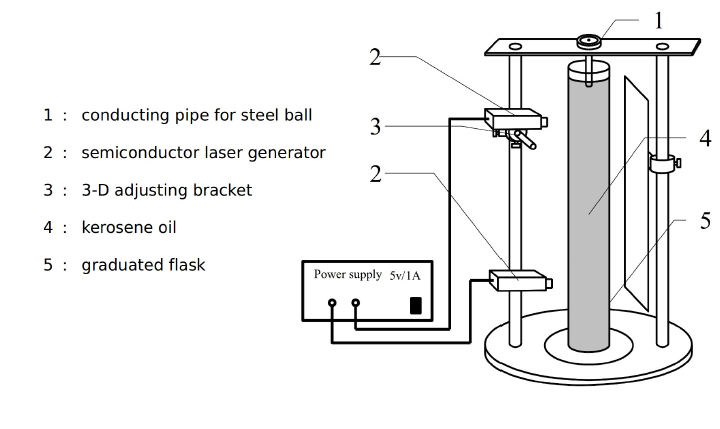
\includegraphics[scale=0.8]{P1.jpg}
\caption{Stokes' viscosity measurement apparatus.}
\end{figure}
\subsection{Tools}
The second part is tools, I used the steel ruler and stopwatch to measure the velocity of the falling ball. Electronic scales and micrometer are used to measure the mass of 40 balls and their diameter so that I can calculate its density $\rho_2$. In addition, densimeter is provided for us to measure the castor oil's density $\rho_1$. I also used a calliper to measure the inner diameter D of the graduated flask and read the ambient temperature from the thermometer.
\begin{figure}[H]
\centering
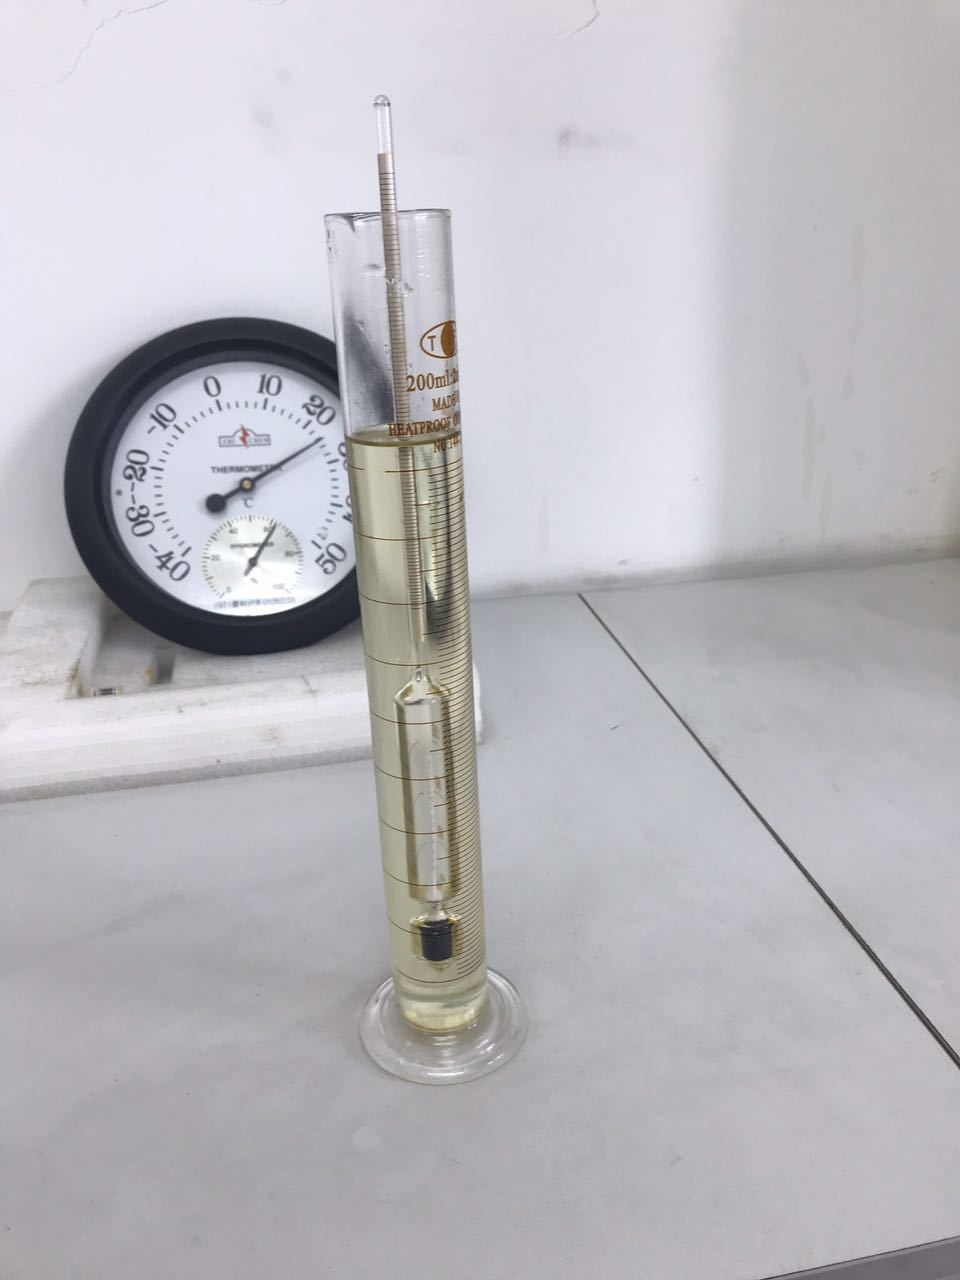
\includegraphics[scale=0.2]{P2.jpg}
\caption{The densimeter}
\end{figure}
\begin{figure}[H]
\centering
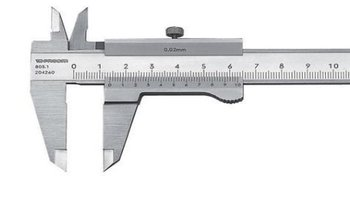
\includegraphics{P3.jpg}
\caption{The calliper}
\end{figure}
\begin{table}[H]
\centering
\begin{tabular}{|c|c|}
\hline
Tools             & Resolution \\ \hline
Steel Ruler       & 1mm        \\ \hline
Stopwatch         & 0.01s      \\ \hline
Micrometer        & 0.004mm    \\ \hline
Calliper          & 0.02mm     \\ \hline
Densimeter        & 0.001g/cm$^3$      \\ \hline
Electronic scales & 0.001g     \\ \hline
Thermometer       & 2$^o$C          \\ \hline
\end{tabular}
\caption{Precision of the measurement instruments}
\end{table}
\section{Measurement Procedure}
\begin{enumerate}
\item Adjustment of the Stokes' viscosity measurement device.
\begin{enumerate}[(1)]
\item Adjust the knobs beneath the base to make the plumb aiming at the center of
the base.
\item Turn on the two lasers, adjust the beams so that they are parallel and aim at
the plumb line.
\item Remove the plumb and place the graduated flask with castor oil at the center of the base.
\item Place the guiding pipe on the top of the viscosity measurement device.
\item Put a metal ball into the pipe and check whether the ball, falling down in the
oil, can blocks the laser beams. If not, repeat Step 1.
\end{enumerate}
\item Measurement of the constant velocity of a falling ball.
\begin{enumerate}[(1)]
\item Measure the vertical distance s between the two laser beams at least three times.
\item Put a metal ball into the guiding pipe. Start the stopwatch when the ball
passes through the first beam, and stop it when it passes through the second
one. Record the time $t$ and repeat the procedure for at least six times.
\end{enumerate}
\item Measurement of the ball density $\rho_2$.
\begin{enumerate}[(1)]
\item Use electronic scales to measure the mass of 40 metal balls. Calculate the
average to find the mass of a single ball.
\item Use a micrometer to measure the diameter of the metal balls. Repeat for ten
times and calculate the average value.
\item Calculate the ball density $\rho_2$.
\end{enumerate}
\item Measure of the density $\rho_1$ of the castor oil by using the provided densimeter (one measurement). Use a calliper to measure the inner diameter $D$ of the graduated flask for six times. Read the ambient temperature from the thermometer placed in the lab.
\item Calculate the value of viscosity coefficient $\eta$ using equation (8).
\end{enumerate}
\section{Calculation and Results}
\subsection{Measurement Results}
\subsubsection{Distance between Two Laser Beams}
I used a steel ruler to measure the distance between two laser beams.  
\begin{table}[H]
\centering
\begin{tabular}{|c|c|c|c|}
\hline
  & initial reading & ending reading & distance S{[}mm{]}$\pm$1{[}mm{]} \\ \hline
$S_1$ & 0.000           & 159.5          & 159.5              \\ \hline
$S_2$ & 0.000           & 159.0          & 159.0              \\ \hline
$S_3$ & 0.000           & 158.0          & 158.0              \\ \hline
$\bar{S}$ & 0.000           & 158.8          & 158.8             \\ \hline
\end{tabular}
\caption{Distance measurement data}
\end{table}
\subsubsection{Time of the Ball Passing through Two Laser Beams}
I used a stopwatch to measure the time of the ball passing through two laser beams.
\begin{table}[H]
\centering
\begin{tabular}{|c|c|}
\hline
\multicolumn{2}{|c|}{time t{[}s{]}$\pm$0.01{[}s{]}} \\ \hline
$t_1$                    & 7.66                    \\ \hline
$t_2$                    & 7.68                    \\ \hline
$t_3$                    & 7.69                    \\ \hline
$t_4$                    & 7.78                    \\ \hline
$t_5$                    & 7.62                    \\ \hline
$t_6$                    & 7.85                    \\ \hline
$\bar{t}$                   & 7.71                    \\ \hline
\end{tabular}
\caption{Time measurement data}
\end{table}
\subsubsection{The Diameters of the Balls}
Micrometer is used to measure the diameters of the balls. I recorded the initial readings and measured 10 balls.
\begin{table}[H]
\centering
\begin{tabular}{|c|c|c|}
\hline
\multicolumn{2}{|c|}{initial reading{[}mm{]}} & 0.005                           \\ \hline
                 & end reading                & diameter d{[}mm{]}$\pm$0.004{[}mm{]} \\ \hline
$d_1$                & 2.000                      & 1.995                           \\ \hline
$d_2$                & 1.995                      & 1.990                           \\ \hline
$d_3$                & 1.990                      & 1.985                           \\ \hline
$d_4$                & 1.990                      & 1.985                           \\ \hline
$d_5$                & 1.995                      & 1.990                           \\ \hline
$d_6$                & 2.005                      & 2.000                           \\ \hline
$d_7$                & 1.995                      & 1.990                           \\ \hline
$d_8$                & 1.990                      & 1.985                           \\ \hline
$d_9$                & 1.995                      & 1.990                           \\ \hline
$d_{10}$                & 2.000                      & 1.995                           \\ \hline
$\bar{d}$                & 1.996                      & 1.991                           \\ \hline
\end{tabular}
\caption{Measurement data for the diameters of the balls}
\end{table}
\subsubsection{Inner Diameter of the Flask}
I used a calliper to measure the inner diameter of the flask. Since the inner shape of the flask is not a standard circle, I measured 6 times
\begin{table}[H]
\centering
\begin{tabular}{|c|c|}
\hline
\multicolumn{2}{|c|}{diameter D{[}mm{]}$\pm$0.02{[}mm{]}} \\ \hline
$D_1$                       & 59.00                      \\ \hline
$D_2$                       & 60.10                      \\ \hline
$D_3$                       & 58.88                      \\ \hline
$D_4$                       & 59.68                      \\ \hline
$D_5$                       & 60.32                      \\ \hline
$D_6$                       & 58.82                      \\ \hline
$\bar{D}$                       & 59.47                      \\ \hline
\end{tabular}
\caption{Measurement data for the inner diameter of the flask}
\end{table}
\subsubsection{Other Physical Quantities}
I also measured the castor oil's density, the mass of 40 metal balls, temperature in the lab once, and the acceleration due to gravity is given to us.
\begin{table}[H]
\centering
\begin{tabular}{|c|}
\hline
density of the castor oil {[}g/cm$^3${]}$\pm$0.001{[}g/cm$^3${]}    \\ \hline
0.955                                          \\ \hline
mass of 40 metal balls m{[}g{]}$\pm$0.001{[}g{]}      \\ \hline
1.358                                          \\ \hline
temperature in the lab T{[}$^o$C{]$\pm$}2{[}$^o$C{]}          \\ \hline
26                                             \\ \hline
acceleration due to gravity in the lab g{[}m/s$^2${]} \\ \hline
9.794                                          \\ \hline
\end{tabular}
\caption{Values of other physical quantities}
\end{table}
\subsection{Calculation of Viscosity Coefficient $\eta$}
$$R_c=0.5\times \bar{D}=29.74[mm]=2.974\times 10^{-2}[m]$$
$$R=0.5\times \bar{d}=0.9955[mm]=9.955\times 10^{-4}[m]$$
$$t=7.71[s]$$
$$S=158.8[mm]=1.588\times10^{-1}[m]$$
$$\rho_1=0.955[g/cm^3]=0.955\times 10^3[kg/m^3]$$
$$\rho_2=\frac{3m}{160\pi R^3}=8.215[g/cm^3]=8.215\times 10^3[kg/m^3]$$
$$\eta=\frac{2}{9}R^2\frac{(\rho_2-\rho_1)gt}{(1+2.4\frac{R}{R_c})s}=7.003\times10^{-1}[kg/(m\cdot{s})]$$
\section{Measurement Uncertainty Analysis}
\subsection{Multiple Measurements Yield to Type A Uncertainty}
For multiple measurements' uncertainty:
$$\bar{X}=\frac{1}{n}\sum_{i=1}^nx_i$$
$$S_X=\sqrt{\frac{1}{n-1}\sum_{i=1}^n(x_i-\bar{X})^2}$$  
$$\bigtriangleup_A=\frac{S_Xt_{0.95}}{\sqrt{n}}$$
The value of $t_0.95$ and $\frac{t_{0.95}}{\sqrt{n}}$ are giving in Table 7 
\begin{table}[H]
\centering
\begin{tabular}{|l|l|l|l|l|l|l|l|l|l|l|l|}
\hline
n                         & 3    & 4    & 5     & 6    & 7     & 8     & 9     & 10    & 15    & 20    & $\ge100$   \\ \hline
$t_0.95$                  & 4.30 & 3.18 & 2.78  & 2.57 & 2.45  & 2.36  & 2.31  & 2.26  & 2.14  & 2.09  & $\le1.97$  \\ \hline
$\frac{t_0.95}{\sqrt{n}}$ & 2.48 & 1.59 & 1.204 & 1.05 & 0.926 & 0.834 & 0.770 & 0.715 & 0.553 & 0.467 & $\le0.139$ \\ \hline
\end{tabular}
\caption{The values of $t_{0.95}$ and $\frac{t_{0.95}}{\sqrt{n}}$}
\end{table}
\subsubsection{Type A Uncertainty of Distance S}
$$\bar{S}=\frac{1}{3}\sum_{i=1}^3{S_i}=158.8[mm]$$
$$S_S=\sqrt{\frac{1}{2}\sum_{i=1}^3{(S_i-158.8)^2}}=0.7638$$
$$\bigtriangleup_A=2.48S_S=1.894[mm]$$
\subsubsection{Type A Uncertainty of Time t}
$$\bar{t}=\frac{1}{6}\sum_{i=1}^6{S_i}=7.71[s]$$
$$S_t=\sqrt{\frac{1}{5}\sum_{i=1}^6{(S_i-7.71)^2}}=0.08524$$
$$\bigtriangleup_A=1.05S_t=0.08951[s]$$
\subsubsection{Type A Uncertainty of Balls' Diameters}
$$\bar{d}=\frac{1}{10}\sum_{i=1}^10{S_i}=1.991[mm]$$
$$S_d=\sqrt{\frac{1}{9}\sum_{i=1}^10{(S_i-1.991)^2}}=4.792\times10^{-3}$$
$$\bigtriangleup_A=0.715S_d=3.555\times10^{-3}[mm]$$
\subsubsection{Type A Uncertainty of Flask's Inner Diameters}
$$\bar{D}=\frac{1}{6}\sum_{i=1}^6{S_i}=59.47[mm]$$
$$S_d=\sqrt{\frac{1}{5}\sum_{i=1}^6{(S_i-7.71)^2}}=0.6565$$
$$\bigtriangleup_A=1.05S_d=0.6893[mm]$$
\subsection{Uncertainty of Directly Measured Physical Quantities}
\subsubsection{Uncertainty of Distance S}
Since the steel ruler's resolution is $\pm1[mm]$, its data's $\bigtriangleup_B$=1[mm]
$$u=\sqrt{\bigtriangleup_B^2+\bigtriangleup_A^2}=\sqrt{1+1.894^2}=2.142[mm]=2.142\times10^{-3}[m]$$ 
$$u_r=\frac{u}{\bar{S}}\times100\%=\frac{2.142\times10^{-3}}{1.588\times10^{-1}}\times100\%=1.34\%$$
\subsubsection{Uncertainty of Time t}
Since the stopwatch's resolution is $\pm0.011[s]$, its data's $\bigtriangleup_B$=0.01[s]
$$u=\sqrt{\bigtriangleup_B^2+\bigtriangleup_A^2}=\sqrt{0.01^2+0.08524^2}=8.582\times10^{-2}[s]$$
$$u_r=\frac{u}{\bar{t}}\times100\%=\frac{8.582\times10^{-2}}{7.71}\times100\%=1.11\%$$
\subsubsection{Uncertainty of Ball's Diameter d}
Since the micrometer's resolution is $\pm0.004[mm]$, its data's $\bigtriangleup_B$=0.004[mm]
$$u=\sqrt{\bigtriangleup_B^2+\bigtriangleup_A^2}=\sqrt{0.004^2+(3.555\times10^{-3})^2}=5.351\times10^{-3}[mm]=5.351\times10^{-6}[m]$$ 
$$u_r=\frac{u}{\bar{d}}\times100\%=\frac{5.351\times10^{-6}}{1.991\times10^{-3}}\times100\%=0.27\%$$
\subsubsection{Uncertainty of Flask's Inner Diameter D}
Since the calliper's resolution is $\pm0.02[mm]$, its data's $\bigtriangleup_B$=0.02[mm]
$$u=\sqrt{\bigtriangleup_B^2+\bigtriangleup_A^2}=\sqrt{0.02^2+0.6893^2}=0.6896[mm]=6.896\times10^{-4}[m]$$ 
$$u_r=\frac{u}{\bar{D}}\times100\%=\frac{6.896\times10^{-4}}{5.947\times10^{-2}}\times100\%=1.16\%$$
\begin{table}[]
\centering
\begin{tabular}{|c|c|c|c|}
\hline
Physical quantities      & Measurement &Uncertainty & Relative uncertainty      \\ \hline
Distance S{[}m{]}        &  $1.588\times10^{-1}$     &$2.142\times10^{-3}$   & 1.34\% \\ \hline
Time t{[}s{]}            & 7.71  & $8.582\times10^{-2}$  & 1.11\% \\ \hline
Ball's diameter d{[}m{]} &  $1.991\times10^{-3}$     & $5.351\times10^{-6}$  & 0.27\% \\ \hline
Inner diameter D{[}m{]}  &  $5.947\times10^{-2}$     & $6.896\times10^{-4}$  & 1.16\% \\ \hline
$\rho_1{[}kg/m^3{]}$                       &  955     &  1 & 0.1\%  \\ \hline
40 ball's mass {[}kg{]}         &   $1.358\times10^{-3}$    &  $10^{-6}$ & 0.07\% \\ \hline
Lab Temperature T {[}$^oC${]}       & 26    & 2 & 7.69\% \\ \hline
\end{tabular}
\caption{Uncertainty of directly measured physical quantities}
\end{table}
\subsection{Uncertainty of Indirectly Measured Physical Quantities}
\subsubsection{Uncertainty of the Ball's Radius}
$$R=\frac{d}{2}$$
$$u_R=\sqrt{(\frac{\partial{r}}{\partial{d}}u_d)^2}=\frac{u_d}{2}=2.676\times10^{-6}[m]$$
\subsubsection{Uncertainty of the Flask's Radius}
$$R_c=\frac{D}{2}$$
$$u_{R_c}=\sqrt{(\frac{\partial{R_c}}{\partial{D}}u_D)^2}=\frac{u_D}{2}=3.448\times10^{-4}[m]$$
\subsubsection{Uncertainty of the Metal's Density}
$$\rho_2=\frac{3m}{160\pi R^3}$$
$$u_{\rho_2}=\sqrt{(\frac{\partial{\rho_2}}{\partial{m}}u_m)^2+(\frac{\partial{\rho_2}}{\partial{R}}u_R)^2}=\sqrt{(\frac{3}{160\pi{R^3}}u_m)^2+(\frac{-9m}{160\pi{R^4}}u_R)^2}=89.72[kg/m^3]$$
\subsubsection{Uncertainty of the Coefficient $\eta$}
$$\eta=\frac{2}{9}R^2\frac{(\rho_2-\rho_1)gt}{(1+2.4\frac{R}{R_c})s}$$
$$u_{\eta}=\sqrt{(\frac{\partial{\eta}}{\partial{R}}u_R)^2+(\frac{\partial{\eta}}{\partial{R_c}}u_{R_c})^2+(\frac{\partial{\eta}}{\partial{t}}u_t)^2+(\frac{\partial{\eta}}{\partial{S}}u_S)^2+(\frac{\partial{\eta}}{\partial{\rho_1}}u_{\rho_1})^2+(\frac{\partial{\eta}}{\partial{\rho_2}}u_{\rho_2})^2}$$
$$\frac{\partial{\eta}}{\partial{R}}u_R=\frac{2(\rho_2-\rho_1)gt}{9S}\cdot\frac{2R(1+\frac{2.4R}{R_c})-R^2\cdot\frac{2.4}{R_c}}{(1+\frac{2.4R}{R_c})^2}\cdot{u_R}=3.643\times10^{-3}$$
$$\frac{\partial{\eta}}{\partial{R_c}}u_{R_c}=\frac{2(\rho_2-\rho_1)R^2gt}{9S}\cdot\frac{2.4R}{(R_c+2.4R)^2}\cdot{u_{R_c}}=6.067\times10^{-4}$$
$$\frac{\partial{\eta}}{\partial{t}}u_{t}=\frac{2}{9}R^2\frac{(\rho_2-\rho_1)g}{(1+2.4\frac{R}{R_c})s}\cdot{u_t}=7.095\times10^{-3}$$
$$\frac{\partial{\eta}}{\partial{S}}u_S=-\frac{2}{9}R^2\frac{(\rho_2-\rho_1)gt}{(1+2.4\frac{R}{R_c})s^2}u_s=9.493\times10^{-3}$$
$$\frac{\partial{\eta}}{\partial{\rho_1}}u_{\rho_1}=-\frac{2}{9}R^2\frac{gt}{(1+2.4\frac{R}{R_c})s}u_{\rho_1}=-8.779\times10^{-5}$$
$$\frac{\partial{\eta}}{\partial{\rho_2}}u_{\rho_2}=\frac{2}{9}R^2\frac{gt}{(1+2.4\frac{R}{R_c})s}u_{\rho_2}=7.877\times10^{-3}$$
$$u_{\eta}=0.0147[kg/(m\cdot{s})]$$
$$u_{r_{\eta}}=\frac{u_{\eta}}{\eta}\times100\%=\frac{0.0147}{7.003\times10^{-1}}\times100\%=2.1\%$$
\begin{table}[H]
\centering
\begin{tabular}{|c|c|c|c|}
\hline
Physical quantities    & Measurement & Uncertainty & Relative uncertainty \\ \hline
Ball's radius R[m]       &    $9.955\times10^{-4}$         &   $2.676\times10^{-6}$          & 0.26\%                     \\ \hline
Flask's inner radius R[m] & $2.974\times10^{-2}$            &    $3.448\times10^{-4}$         & 1.16\%                     \\ \hline
Ball's density[$kg/m^3$]         &    8215         &   $89.72$          &                     1.09\% \\ \hline
Coefficient[$kg/(m\cdot{s})$]            &   $7.003\times10^{-1}$          &            0.0147 &   2.10\%                   \\ \hline
\end{tabular}
\caption{Uncertainty of indirectly measured physical quantities}
\end{table}
\section{Conclusion and Discussion}
\subsection{Conclusion}
In the exercise, Stokes' method is used to measure the viscosity coefficient $\eta$, and my final result is $7.003\times10^{-1}\pm1.47\times10^{-2}[kg/(m\cdot{s})]$ with relative uncertainty equals 2.1\%. 
\par The Stokes' method is based on Stokes' Law established by an English scientist Sir George G Stokes: When a spherical body moves down through an infinite column of highly viscous liquid, it drags the layer of the liquid in contact with it. As a result, the body experiences a retarding force and we can use the force as an intermediate quantity to measure $\eta$.
\par After the exercise, I become familiar with fluid's viscosity and Stokes' method, a basic and simple way to calculate the viscosity. In addition, I also learned how to use micrometer and densimeter to calculate micro diameter and fluid's density.
\subsection{Discussion}
\subsubsection{Measurement of Non-transparent Fluid's Viscosity}
\par However, our method can't be easily applied to measure the $\eta$ of non-transparent fluid because I can't measure the time for the metal ball to pass through the two laser beams. I find other three methods to measure the fluid viscosity.
\begin{enumerate}
\item Use the rotational viscometer to measure the torque required to turn an object in the fluid, which is a function of $\eta$, and $\eta$ can be calculating as following formula:
\begin{figure}[H]
\centering
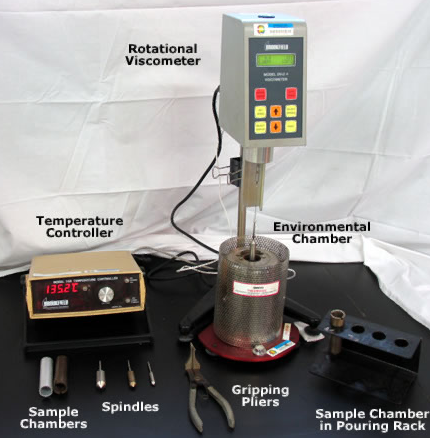
\includegraphics{P4.jpg}
\caption{The rotational viscometer}
\end{figure}
$$\eta=\frac{\tau}{\gamma}$$
{\centering \footnotesize  $\tau$:shear stress\\$\gamma$:shear rate\\
} 
$$\tau=\frac{T}{2\pi{R_s^2L}}$$
{\centering \footnotesize  $T$:the torque \\$R_s$:spindle radius\\$L$:effective spindle length\\} 
$$\gamma=\frac{2\omega{R_s^2R_c^2}}{x^2(R_s^2-R_c^2)}$$
{\centering \footnotesize  $\omega$:rotational speed \\$x$:radial location where shear rate is being calculated\\} 
\item We can use vibrational viscometer ,which operating by measuring the damping of an oscillating electromechanical resonator immersed in a fluid whose viscosity is to be determined.The resonator generally oscillates in torsion or transversely. The higher the viscosity, the larger the damping imposed on the resonator. The resonator's damping may be measured by one of several methods:
\begin{enumerate}[(1)]
\item Measuring the power input necessary to keep the oscillator vibrating at a constant amplitude. The higher the viscosity, the more power is needed to maintain the amplitude of oscillation.
\item Measuring the decay time of the oscillation once the excitation is switched off. The higher the viscosity, the faster the signal decays.
\item Measuring the frequency of the resonator as a function of phase angle between excitation and response waveforms. The higher the viscosity, the larger the frequency change for a given phase change.
\end{enumerate}
\item Rectangular-slit viscometer can also be used to measure the viscosity.The basic design of a rectangular-slit viscometer consists of a rectangular, slit channel with uniform cross-sectional area. A test liquid is pumped at a constant flow rate through this channel. Multiple pressure sensors flush mounted at linear distances along the stream-wise direction measure pressure drop as depicted in Figure 5.
\begin{figure}[H]
\centering
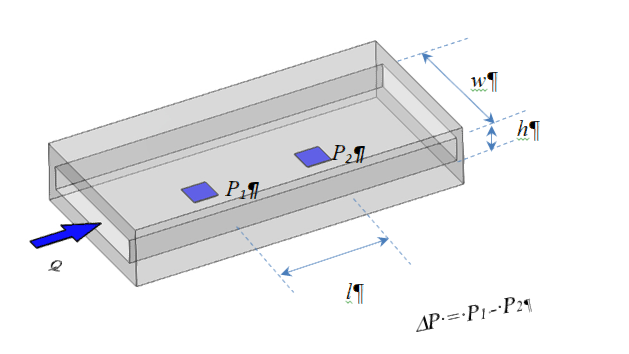
\includegraphics{P5.jpg}
\caption{Rectangular-slit viscometer}
\end{figure}
The slit viscometer is based on the fundamental principle that a viscous liquid resists flow, exhibiting a decreasing pressure along the length of the slit. The pressure decrease or drop $\bigtriangleup{P}$ is correlated with the shear stress at the wall boundary. The apparent shear rate is directly related to the flow rate and the dimension of the slit. The apparent shear rate, the shear stress, and the apparent viscosity are calculated:
$$\gamma=\frac{6Q}{w{h^2}}$$
{\centering \footnotesize  $\gamma$:apparent shear rate\\$Q$:flow rate\\$w$:width of the flow channel\\$h$:depth of the flow channel\\
} 
$$\sigma=\frac{hw\bigtriangleup{P}}{2(w+h)l}$$
{\centering \footnotesize  $\bigtriangleup{P}$:pressure difference between the leading pressure sensor and the last pressure sensor\\$l$:the distance between the leading pressure sensor and the last pressure sensor\\
} 
$$\tau_a=\frac{\sigma}{\gamma}$$
To determine the viscosity of a liquid, pump the liquid sample to flow through the slit channel at a constant flow rate and measure the pressure drop. Following these equations, calculate the apparent viscosity for the apparent shear rate. For a Newtonian liquid, the apparent viscosity is the same as the true viscosity and the single shear rate measurement is sufficient. For non-Newtonian liquids, the apparent viscosity is not true viscosity. In order to obtain true viscosity, measure the apparent viscosities at multiple apparent shear rates. Then calculate true viscosities, $\tau$, at various shear rates using Weissenberg-Rabinowitsch-Mooney correction factor:
$$\frac{1}{\tau}=\frac{1}{2\tau_a}(2+\frac{dln\gamma}{dln\sigma})$$
\end{enumerate}
\subsubsection{Error Analysis}
\begin{enumerate}
\item The biggest cause for error in measurement is time. Since I clicked the stopwatch when I saw the ball block the laser, it's very inaccurate for my eyes to determine the time.
\item The second cause is the temperature in the lab. Even though I have measured the temperature in the lab through thermometer, the temperature is still changing in the lab and the thermometer also has a quite big relative uncertainty. Since fluid's viscosity is determined by temperature and its type, the temperature could have a significant impact on the fluid's viscosity.
\item We measure the mass of forty metal balls at one time because their mass is about 1.3[g]. If I measure one or ten balls at a time, the significant figures may not be enough for me to get a precise value of one ball's mass. However, since I only measure the time for six times, the mass of the six balls may be slightly different from the 40 balls, which might cause error.
\item Since the flask is not a standard circle, I measure its inner diameter for six times but I think it's not enough because their relative uncertainty is big.
\end{enumerate}
\subsubsection{Improvements and Suggestions}
\begin{enumerate}
\item Use laser sensors and a computer system to measure the time travelled. When the laser is blocked it will start timing and stop until another laser is blocked. I think it'll be more accurate.
\item When I use the steel ruler to measure the distance S, my initial reading is always 0.000, which is not good for measurement because the 0 point of the ruler may be not accurate. I should use different initial reading when I use a steel ruler later. 
\end{enumerate}
\section{Data Sheet}
Data sheet is attach to the report
\section{Reference}
\begin{enumerate}
\item Young, H.D., Freedman R.A. University Physics. ,12.1, 12.3, 12.6.
\item Qin Tian, Zeng Ming, Zhao Xijian, Krzyzosiak,M. Lab Manual of Exercise 2.
\item Qin Tian, Zeng Ming, Zhao Xijian, Krzyzosiak,M. Handbook-Uncertainty Analysis.
\item https://www.quora.com/What-are-the-different-methods-to-measure-the-viscosity-of-
fluid
\item https://en.wikipedia.org/wiki/Viscometer
\end{enumerate}

\end{document}